To see how the our previous extrapolation methods impact the evaluation of \n{6}{Li}, we will evaluate the nucleus using both the absolute and the difference based extrapolation framework and all the different training modes introduced in \autoref{chap:extended}. For the evaluation, NCSM sequences of \n{6}{Li} are only available up to $N_\mathrm{max} = 10$. The evaluation will thus be done for a maximum $N_\mathrm{max}$ of 8 and 10. The resulting evaluation can be seen in \autoref{fig:eval_li6}.

First, we want to look at the absolute based extrapolation. Here, the unmodified training mode results in a plausible extrapolation of the given NCSM sequences, satisfying the variational boundary condition even for the highest $N_\mathrm{max}$ of 10. Also, the resulting predictions for the ground-state energy are very consistent across the different $N_\mathrm{max}$ values, in contrast to the classical extrapolations, which provide a higher prediction than our framework for $N_\mathrm{max} = 8$ but a lower prediction than our framework for $N_\mathrm{max} = 10$.

In contrast to the unmodified training mode, the $N_\mathrm{max}$-limitation training mode provides no significant different result. The results of this training mode are very unconsistent, as they predict a lower value for $N_\mathrm{8}$ and $\eta = 0.04$ than the unmodified training mode, but a higher value for all other $N_\mathrm{max}$. This is the behaviour we already encountered in \autoref{chap:extended}.

Surprisingly, the SRG-filter training mode produces a very unreasonably high extrapolation for all $N_\mathrm{max}$ values. The extrapolations produced by this training mode are very close to the variational boundaries of $N_\mathrm{max} = 10$, but since the NCSM sequences of \n{6}{Li} are not sufficiently converged until this $N_\mathrm{max}$ value, the variational boundary does not provide a good comparison for the extrapolated ground-state energy.

The extrapolations for the flow parameter \srg{0.08} have a smaller uncertainty than those for the flow parameter \srg{0.04}. This is not an effect that we have seen that strong in the evaluation of the three nuclei used in training in \autoref{chap:extended}. This may originate from the more converged sequences that are present in the $\eta = \srg{0.08}$ data set, which also explains the more consistent classical extrapolations across the $N_\mathrm{max}$ values, which are usually very dependant on the degree of convergence of the sequences.

\begin{figure}[H]
  \caption{Evaluation results for the \n{6}{Li} nucleus using the absolute \textbf{(a)} and the difference based extrapolation \textbf{(b)}. The shown training modes are, in order from left to right, the unmodified training mode for comparison, the $N_\mathrm{max}$-limitation training mode and the SRG-filter training mode. For each nucleus and each flow parameter, the NCSM sequences are shown on the left and the extrapolations for a given maximum $N_\mathrm{max}$ on the right. For each maximum $N_\mathrm{max}$, the variational boundary is shown as a dotted line, and the classical extrapolations are shown as red ticks.}

  \label{fig:eval_li6}
  \begin{subfigure}{\textwidth}
    \caption{}
    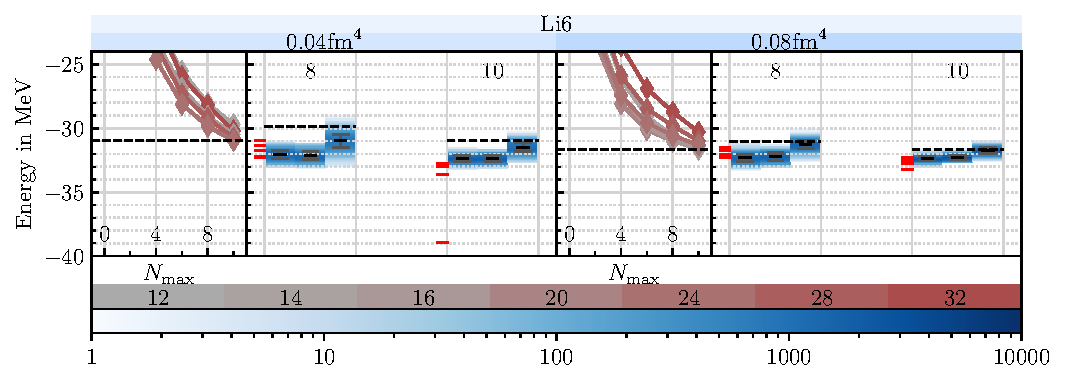
\includegraphics[width=\textwidth]{media/li6_evaluation_abs.pdf}
  \end{subfigure}
  \begin{subfigure}{\textwidth}
    \caption{}
    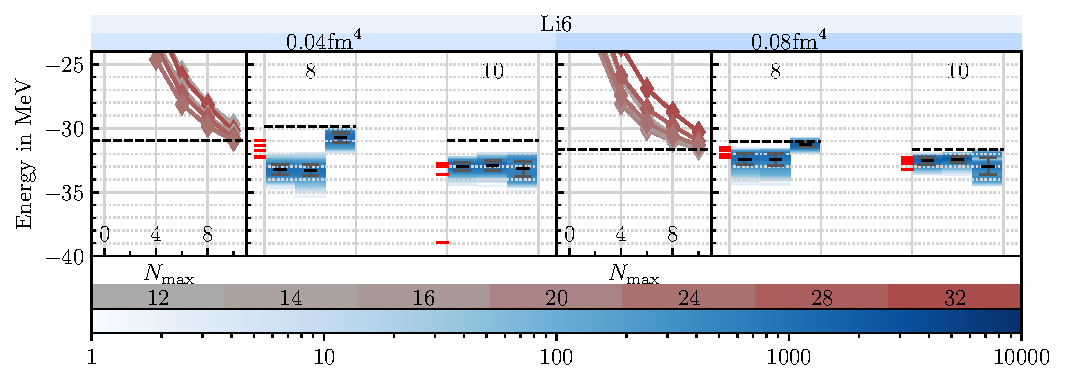
\includegraphics[width=\textwidth]{media/li6_evaluation_diff.pdf}
  \end{subfigure}
\end{figure}

For the difference based extrapolations, the same observations about the unmodified and the $N_\mathrm{max}$-limitation training modes can be made. However, we cannot observe the general improvement of the uncertainties in contrast to the absolute based framework. In fact, the uncertainties are bigger in the evaluation using difference values. In \autoref{chap:diff}, we have found that the difference based extrapolation will produces a larger uncertainty for sequences, which converge uniformly, but are cut off at the higher $N_\mathrm{max}$ values. This effect seems to outweigh the advantages that the difference based framework brings, resulting in an increased uncertainty for \n{6}{Li}. Also, the extrapolation for the SRG-filter training mode is very inconsistent with the observations we made for the absolute based framework. Here, the training mode produces too high values for $N_\mathrm{max} = 8$ but too low values for $N_\mathrm{max} = 10$.
